\chapter{Be candidates}
Astronomical objects used in this work to demonstrate some of the
discussed technologies and methods were Be stars. The target was to
develop a process of finding new candidates in the available
data. Several approaches were considered and two of them are discussed
in the rest of this text. First one utilizes photometric properties
of Be stars, second uses spectra characteristics.


\section{Be stars}

"Classical Be stars are B-type stars close to the main sequence that
exhibit line emission over the photometric spectrum. The excess is
attributed to a circumstellar gaseous component that is commonly
accepted to be in the form of an equatorial disk."

\cite{porter2003classical}.

    \begin{figure}[!htbp]
      \begin{center}
        \leavevmode
        \ifpdf
        \subfloat{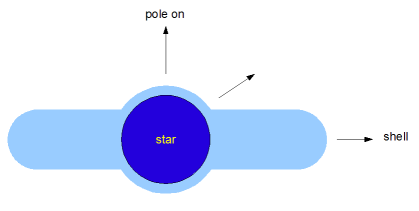
\includegraphics[width=0.5\textwidth]{beStar2}}                
        \subfloat{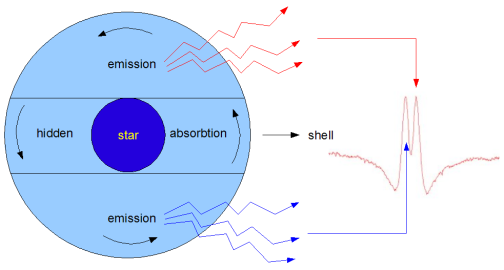
\includegraphics[width=0.5\textwidth]{beStar1}}
        \else
        \includegraphics[bb = 92 86 545 742, height=6in]{beStar}
        \fi
        \caption{Model of a typical Be star \cite{hirata1984star}}
        \label{Figjhk_be_b}
      \end{center}
    \end{figure}

    \begin{figure}[!htbp]
      \begin{center}
        \leavevmode
        \ifpdf
        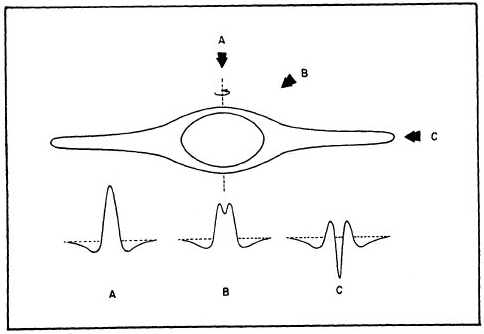
\includegraphics[scale =1]{beSpectra}
        \else
        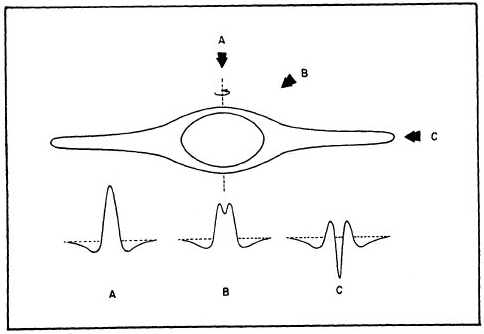
\includegraphics[bb = 92 86 545 742, height=6in]{beSpectra}
        \fi
        \caption{Example of spectra of Be stars based on view angle
          \cite{slettebak1988stars}}
        \label{Figjhk_be_b}
      \end{center}
    \end{figure}

\clearpage

\section{Photometric Data Mining}

% The question I have tried to answer in this chapter was: Is it
% possible to find Be stars candidates based on photometric properties
% only? To answer this question I needed training set of confirmed Be
% stars, set of non Be stars (spectral type B was considered) and some
% Data Mining algorithm to perform classification.

Classification based on photometric properties is very attractive from
several points of view. There are much more aviable phometric then
spectral data and they are easier accesiable. Because they are easier
to gain the disproportion between photometric and spectral data will
probably increase in the future as well. The distinction between Be
and other types of stars also should be theoretically possible since
the Be stars exibits infrared excess correlated to the H$\alpha$
emission \cite{van1995halpha}.

\subsection{Data preprocessing}

I was provided by a list of confirmed Be stars from Academy of Science
Ondřejov. This list consist of 625 manually chosen objects. Data were
correlated with Hipparcos \cite{perryman1997hipparcos} catalog to
obtain RA, DEC and then with 2MASS\cite{2006AJ131.1163S} catalog to
obtain J,H,K Colors using method of multi-cone search in Virtual
Observatory. The second set was acquired from Hipparcos catalog using
following SQL query:

\begin{lstlisting}
  Select * 
  From maincat as m, hipva1 as h 
  Where  (m.HIP=h.HIP )  
  And h.SpType Like 'B%'
\end{lstlisting}

The result was cross-correlated with 2MASS catalog to obtain the same
colors as for the confirmed Be stars. Color digram of this two sets
are on the figure \ref{Figjhk_be_b}

    \begin{figure}[!htbp]
      \begin{center}
        \leavevmode
        \ifpdf
        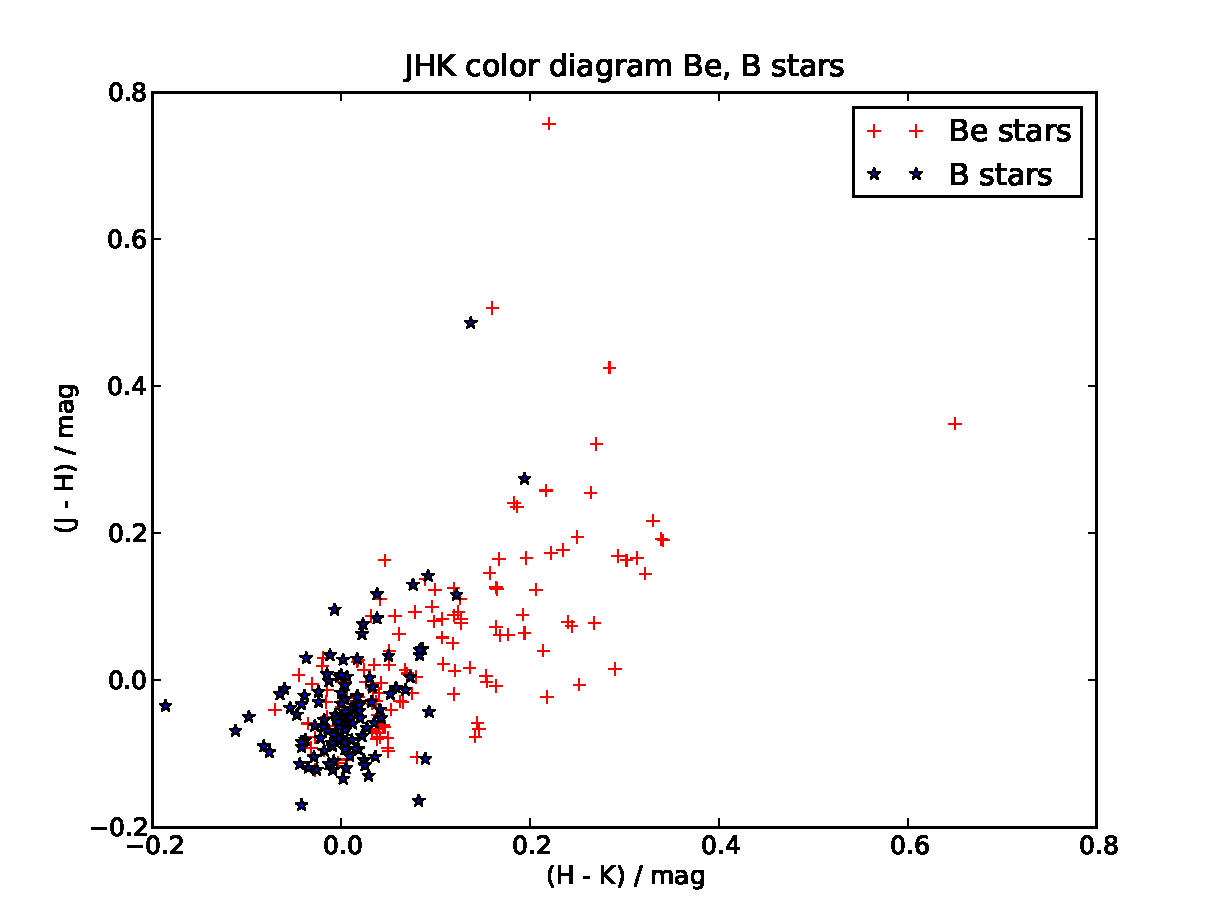
\includegraphics[scale =.6]{jhk_be_b}
        \else
        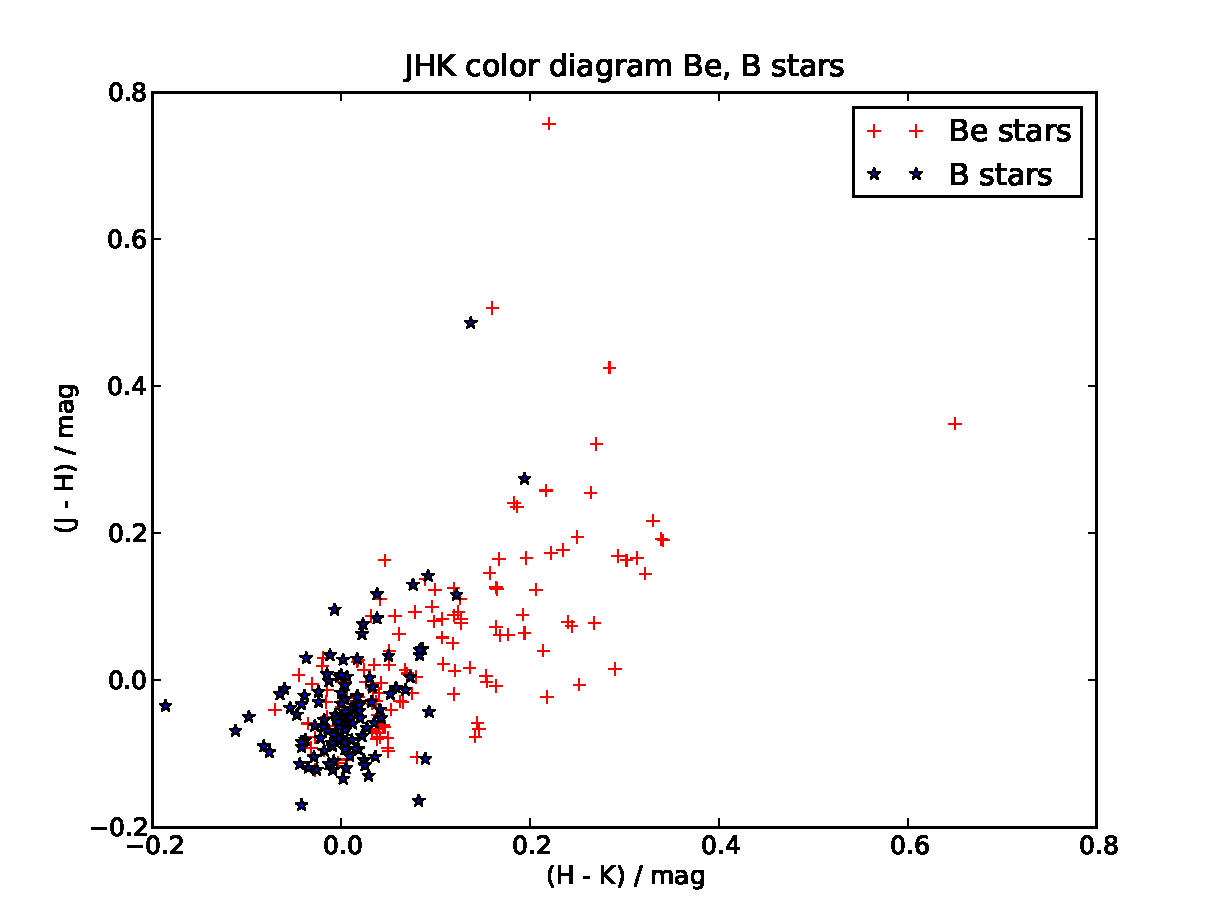
\includegraphics[bb = 92 86 545 742, height=6in]{jhk_be_b}
        \fi
        \caption{Color diagram of confirmed Be stars Vs B stars}
        \label{Figjhk_be_b}
      \end{center}
    \end{figure}

    The uncertainties were computed for each object using propagation
    of error. These errors and depicted on the figure
    \ref{Figjhk_be_b_errors}. Although the uncertainties are
    significant certain trends are presented.

\begin{align*}
  \delta_{(j - h)} = \sqrt{\left(\frac{\partial(j - h) }{\partial
        j}\right)^2\delta_j^2 + \left(\frac{\partial(j - h) }{\partial
        h}\right)^2\delta_h^2} \\
  \frac{\partial(j - h) }{\partial j } = 1,\frac{\partial(j - h)
  }{\partial h } = -1 \\
  \delta_{(j - h)} = \sqrt{\delta_j^2 + \delta_h^2}
\end{align*}


    \begin{figure}[!htbp]
      \begin{center}
        \leavevmode
        \ifpdf
        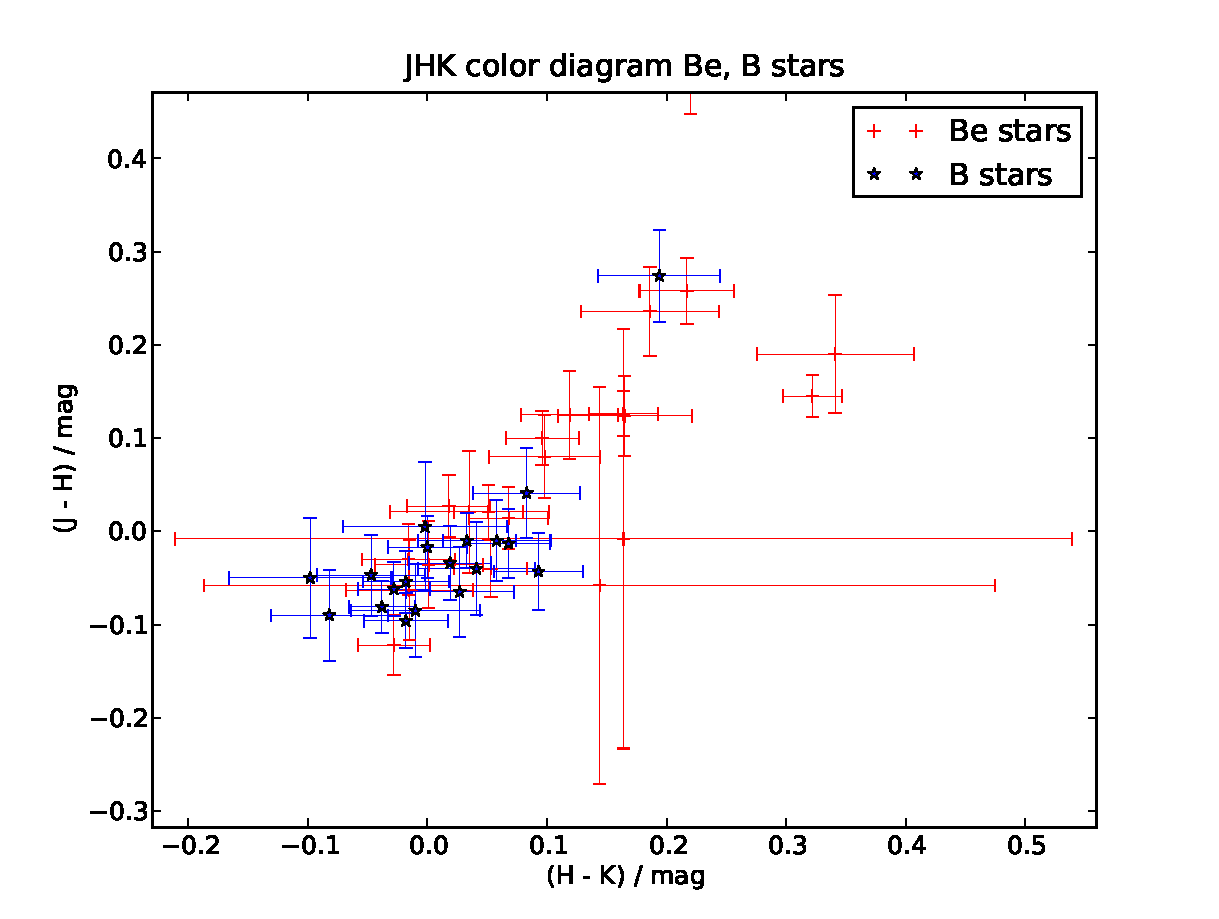
\includegraphics[scale =.6]{jhk_be_b_errors}
        \else
        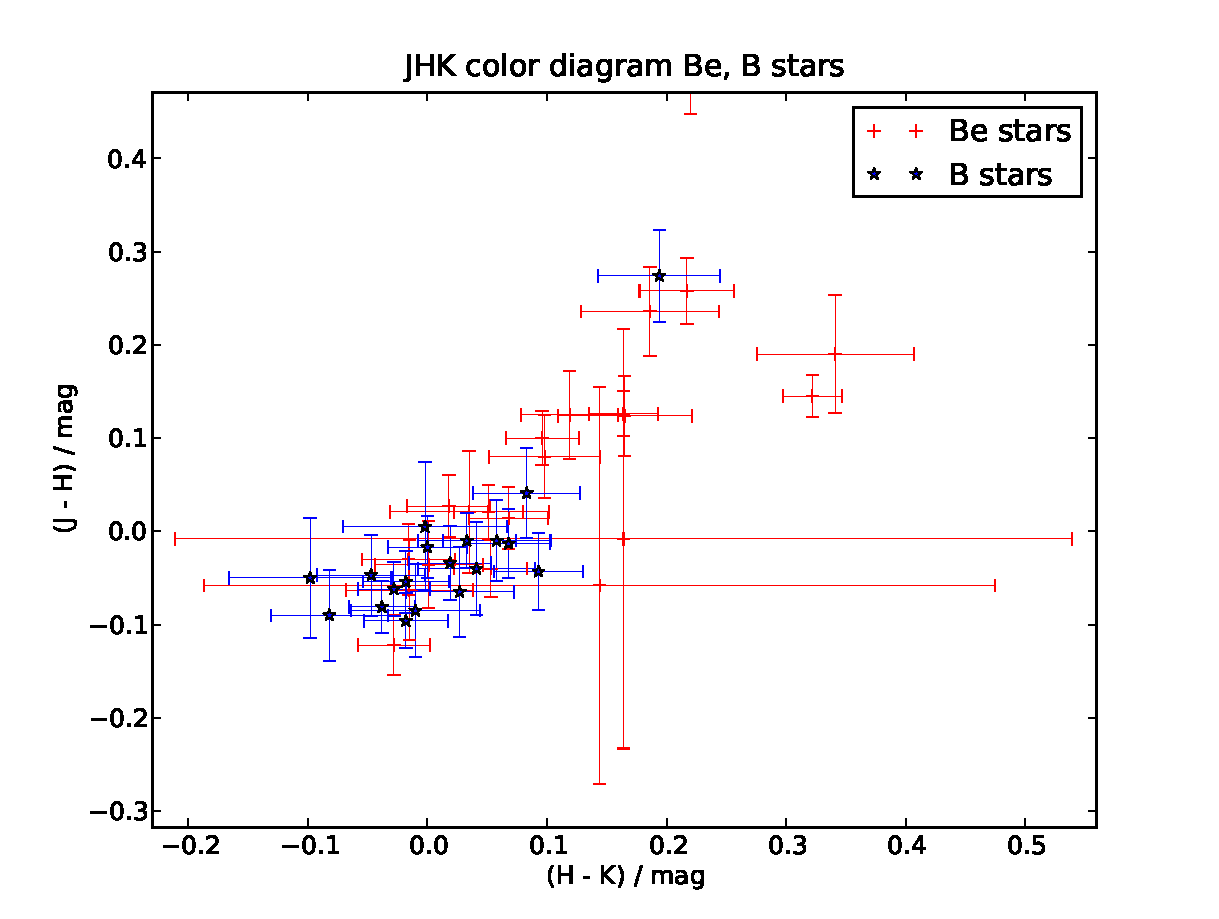
\includegraphics[bb = 92 86 545 742, height=6in]{jhk_be_b_errors}
        \fi
        \caption{Color diagram of confirmed Be stars Vs B stars with errors}
        \label{Figjhk_be_b_errors}
      \end{center}
    \end{figure}

\clearpage


\subsection{Classification}
Data were transformed from original VOTable obtained from Virtual
Observatory tools to arff\footnote{Attribute-Relation File
  Format. Developed by the Machine Learning Project at the Department
  of Computer Science of The University of Waikato.}format used in
Weka Data Mining system. Algorithm C4.5 (J48) was used to perform
actual classification with following result:

\begin{lstlisting}
  Correctly Classified Instances         769               73.0989 %
  Incorrectly Classified Instances       283               26.9011 %
  Kappa statistic                          0.4496
  Mean absolute error                      0.3843
  Root mean squared error                  0.4383
  Relative absolute error                 79.4985 %
  Root relative squared error             89.1648 %
  Total Number of Instances             1052
\end{lstlisting}

As seen on the first row 73 \% from  1052 objects were classified
correctly. More details can be obtained from confusion matrix below.

\begin{lstlisting}
  B   Be   <-- classified as
 304 126 |   B
 157 465 |   Be
\end{lstlisting}

304 of B and 456 of Be stars were classified correctly but 126 of B
and 157 of Be stars were classified incorrectly. In virtue of these
results one should be sceptical if the distinction based only on
photometric properties is significant enough to find relevant new
candidates of Be stars. For this reason more sophisticated (and much
more complicated) approach using spectra analysis was tested.

\section{Spectral Data Mining}
Spectra provide much wider scientific informations over photometric
properties. Spectral lines exibits many distingues features and
astronomers have long tradition of analysing their properties. On the
other side its much complicated ot handle them because of different
characteristics (resolution, calibration, wavelength range, etc). This
is especially true for massive automated processing.  

\subsection{Testing Data}
As testing sample the project SEGUE of SDSS were selected. This
contains 178315 spectra in DR7. Following SQL query was used to
generate the list of URL links for individual FITS files. These files
were then download to local sever using wget command.

\begin{lstlisting}
SELECT  objid,dbo.fGetUrlFitsSpectrum(s.specObjID)                                                           
INTO mydb.segue_1                                                                                     
FROM SpecPhotoAll s, platex p                                                                         
WHERE s.specObjID is not null                                                                         
AND s.plateid = p.plateid                                                                             
AND p.programname LIKE 'segue%'                                                                       
AND specClass = 1
\end{lstlisting}

\subsection{Training Data}
The spectra from Ondřejov Observatory were used as training
sample. Files were downloaded using SSA protocol. The SSA server is
not publically aviable, therefore SSH tunneling was used. Two scripts
for this process were created. First to construct the list of SSA
compliant adresses, the second to analyse acquired response in VOTable
format. Then the spectra were downloaded using wget command. The
fuction for constructing the links based on list of the RA, DEC which
were obtained from Hipparcos catalog using the specification of IDs
from Ondřejov's index.

\begin{lstlisting}
def createQuery(data):
    """ From raw data construct ra, dec """
    """ Convert to degrees """
    for line in data:
        ra = ac.AngularCoordinate(line[0:10]).degrees # convert ra to degrees
        dec = ac.AngularCoordinate(line[-13:-1]).degrees # convert dec to degrees
        ra = line[0]
        dec = line[1]
        ssaTemp = 'http://tvoserver/coude/coude.cgi?c=ssac&n=coude_ssa&REQUEST=queryData&POS=<ra>,<dec>&SIZE=1'
        ssaTemp = ssaTemp.replace('<ra>',"%0.3f" % ra)
        ssaTemp = ssaTemp.replace('<dec>',"%0.3f" % dec)
        ssa.append(ssaTemp)
    return ssa
\end{lstlisting}

The script generate the following output. The same process were used
later for obtaining th sample of non Be stars.

\begin{lstlisting}
http://tvoserver/coude/..._ssa&REQUEST=queryData&POS=83.113,-65.582&SIZE=60
http://tvoserver/coude/..._ssa&REQUEST=queryData&POS=162.537,148.333&SIZE=60
http://tvoserver/coude/..._ssa&REQUEST=queryData&POS=19.907,-73.502&SIZE=60
\end{lstlisting}


\subsubsection{Spectra Reduction}
Because spectra from SDSS and Ondřejov Observatory had different
resolution, reduction was needed. First the parameter CD1\_1 (Coordinate
increment per pixel) had to be obtained form FITS file.


\begin{lstlisting}
  In [1]: hdu = pf.open('sdss_test.fit')
  In [2]: hdu[0].header['CD1_1']
  Out[2]: 0.0001 # SDSS spectrum 
  Out[3]: 0.2567 # Onřejov spectrum
\end{lstlisting}

Spectra in SDSS are stored in logarithmic scale thus the value is
computed as $ 10^{CD1\_1} = 1.00$. The ratio is then
$CD1\_1_{SDSS}/CD1\_1_{OND} = 3.87$. Based on this computation 4
pixels of Ondřejov's spectra were reduced into one. There is the
critical part of the reduction program:

\begin{lstlisting}
 def convolution(f, g):
    """ Convolve two functions"""
    fg = np.convolve(g,f,'same')
    return fg
 def reduce(x,y,bin):
    """ Reduce bin pixel into 1"""
    size = x.size/bin
    l = 0
    xx = x[:x.size-1:bin]
    yy = list()
    for i in range(0,size):
        s = 0
        for j in range(0,bin):
            s = s + y[l]
            l+=1
        yy.append(s/bin)
    return xx, yy
\end{lstlisting}

Prior to binning pixels convolution with gaussian function was
performed on the spectra. Convolution is defined:

\begin{equation}
  \label{eq:convolution}
 (f * g )(t) \stackrel{\mathrm{def}}{=}\ \int_{-\infty}^{\infty} f(\tau)\, g(t - \tau)\, d\tau
\end{equation}
 
Here it was used in it's dicrete form

\begin{equation}
  \label{eq:discreteConvolution}
  (f * g)[n]\ \stackrel{\mathrm{def}}{=}\ \sum_{m=-\infty}^{\infty} f[m]\, g[n - m]
\end{equation}



The result is on the figure


    \begin{figure}[!htbp]
      \begin{center}
        \leavevmode
        \ifpdf
        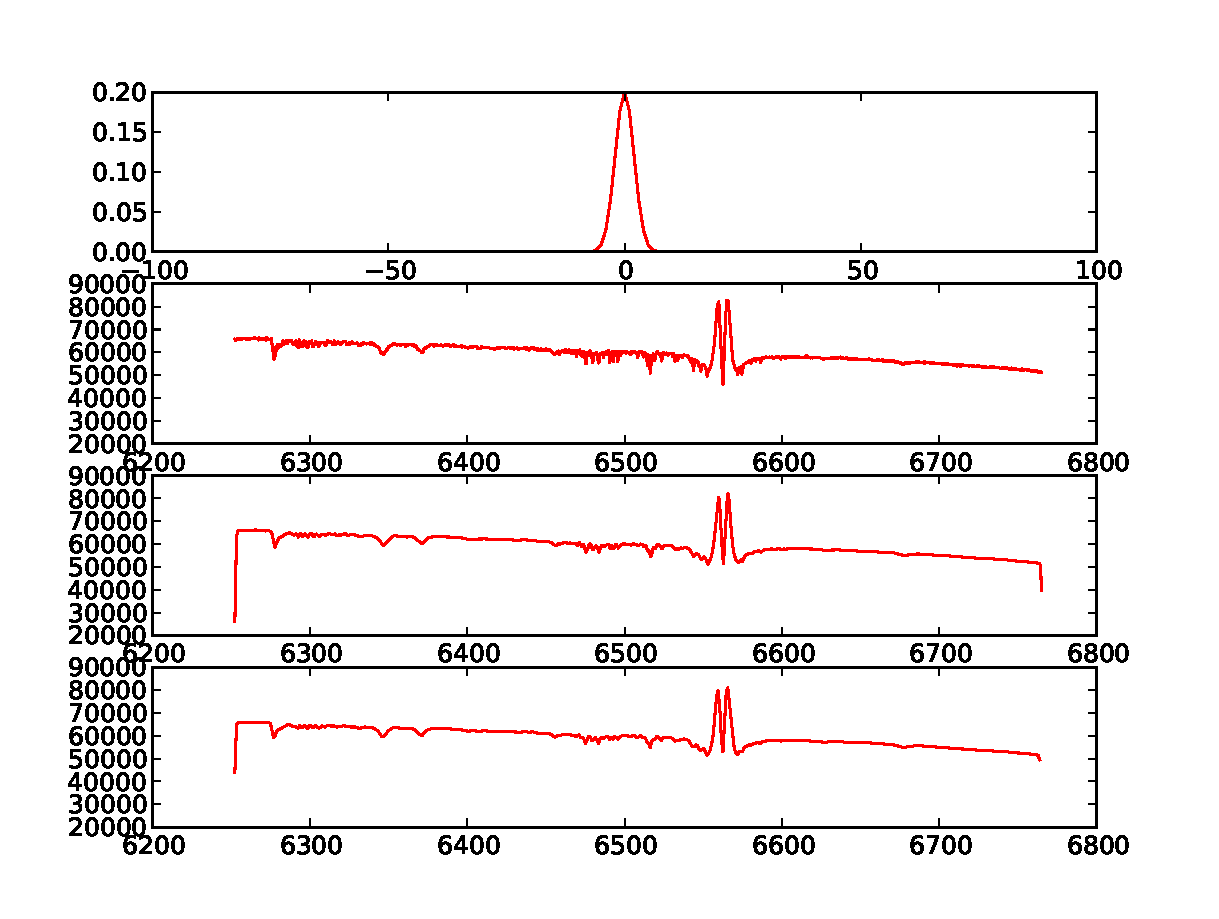
\includegraphics[scale =.8]{convolution}
        \else
        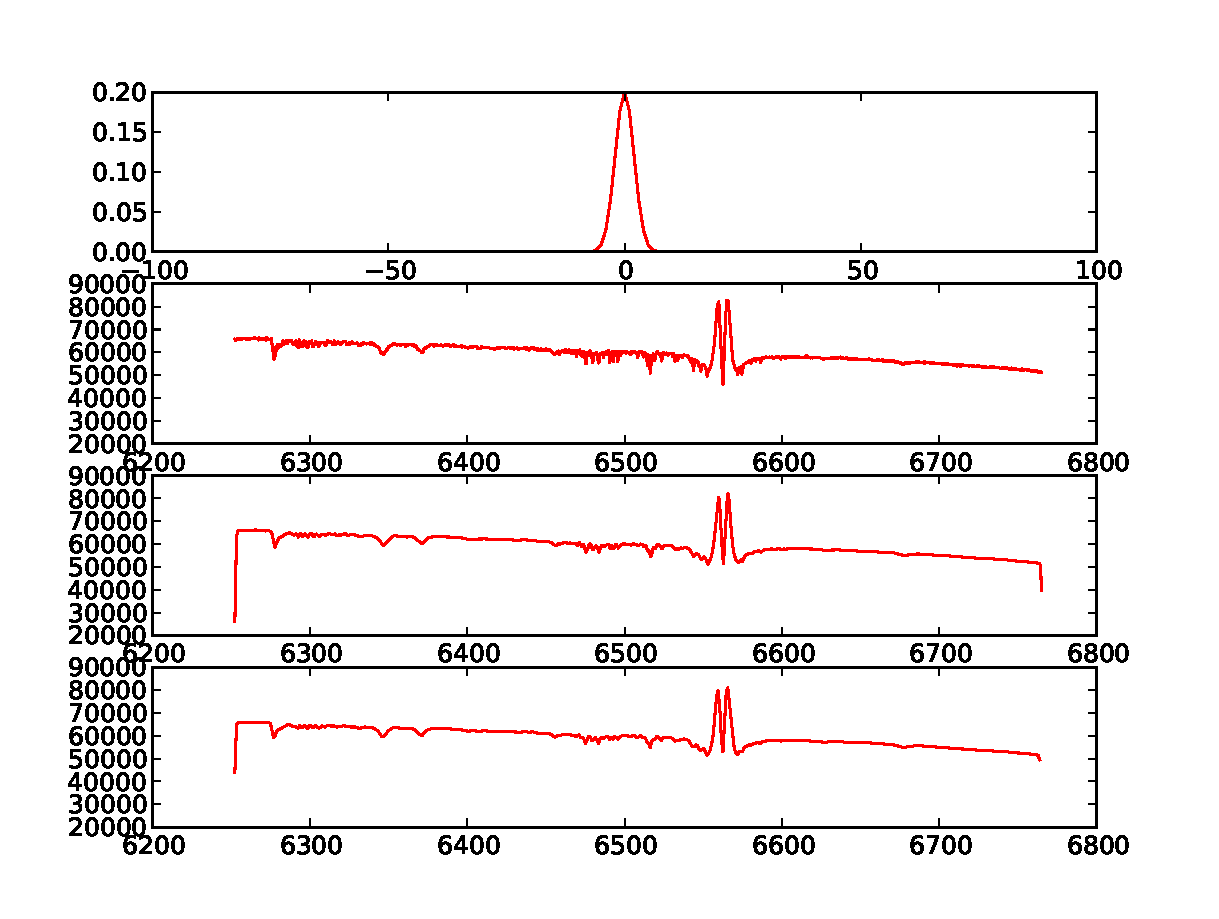
\includegraphics[bb = 92 86 545 742, height=6in]{convolution}
        \fi
        \caption{Reduction of Ondřejov's spectra of the Be star 4
          Hercules. The top figure shows gaussian function used for
          convolution with the structrum, followed by the original
          spectrum then there is a spectrum after convolution with the
          gausian function. The last is the final spectrum after
          reduction.}
        \label{FigReduction}
      \end{center}
    \end{figure}

\clearpage




\subsection{Spectra Lines Characteristics}
As parameters for Data Mining process characteristics value of
H$\alpha$ line were extracted from the spectra. Many possible
characteristics from fitting functions through Wavelets Coefficients
and Eigen Values were discussed with experts. Three parameters were
finally slected. The hight and the width of the H$\alpha$ emission
line and median absolute deviation as a characterization of the noise
level in the spectrum. 


\subsubsection{Normalization}
Spectra from SDSS are normalized but the spectra from Ondřejov are
not. The spectra were devided by it's continuum fit function. This
process ensures the compatibility when comparing different
spectra. Function polyfit from numpy package was used to perfom the
fit. The solution minimizes the squared error:

\begin{align}
  \frac{d}{dq} \sum_{i = 1}^n{(y_i - \operatorname{f}(x_i) )^2} = 0,
\end{align}

where $\operatorname{f}$ is in our case $\operatorname{f}(x) = q_1x +
q_0$.

\subsubsection{The hight of the H$\alpha$ line}
The maximum value in the region of $50\AA$ were extracted from the
spectrum.

\begin{lstlisting}
def getMax(x,y,line,range):
    """ Return maximum value of range in the spectrum"""
    xrange = x[(x < line + range) & (x > line - range)]
    yrange = y[(x < line + range) & (x > line - range)] - 1
    maximum = yrange.max()
    minimum = yrange.min()
    if abs(maximum)  > abs(minimum):
        extrem =  maximum 
    else:
        extrem = minimum 
    return xrange, extrem, sgn
\end{lstlisting}

\subsubsection{The noise level of the spectrum}
The noise in the spectrum contributes to the characteristics of the
spectral lines. As ans estimetor of the noise level the median
absolute deviation was used. It is defined as:

\begin{align}
  \operatorname{mad} = \operatorname{median}_{i}\left(\ \left| X_{i} -
      \operatorname{median}_{j} (X_{j}) \right|\ \right)
\end{align}

\subsubsection{The width of the H$\alpha$ line}
The gaussian function was fitted to the spectral line. First the
robust estimators were computed and used as input parameters for
leastsq\footnote{"leastsqi"s a wrapper around MINPACK’s lmdif and
  lmder algorithms.} method from scipy.opt module, which minimize the
sum of squares.

\begin{align}
  x_0 & = \frac{\operatorname{median}(w_jx_j)}{\sum{w_i}}, \\
  S & = \frac{\operatorname{mad}(x_i - x_0)}{\sum{w_i}}.
\end{align}

Part of the script implementing fitting the gaussian function

\begin{lstlisting}
x0 = np.median(sum(w*x))/sum(w)
S = sum(w*mad((x - x0)))/sum(w)
params = np.array([1, maximum, x0, S], dtype=float)
fit, flag = opt.leastsq(residuals, params, args=(yrange, xrange))
gauss = model(xrange, fit) + 1

def model(t, coeffs):
    return coeffs[0] + coeffs[1] * np.exp( - ((t-coeffs[2])/coeffs[3])**2 )
def residuals(coeffs, y, t):
    return y - model(t, coeffs)
\end{lstlisting}

The final result is on the figure \ref{FigSpecChar1} and
\ref{FigSpecChar2}. The script was adjust to work with SDSS and
Ondřejov's spectra. The whole procedure was performed on all of the
cca 200 000 SDSS spectra and few dozens Ondřejov's spectra resulting
with the ASCII files with the characteristic values used later in Data
Mining process.

   \begin{figure}[!htbp]
      \begin{center}
        \leavevmode
        \ifpdf
        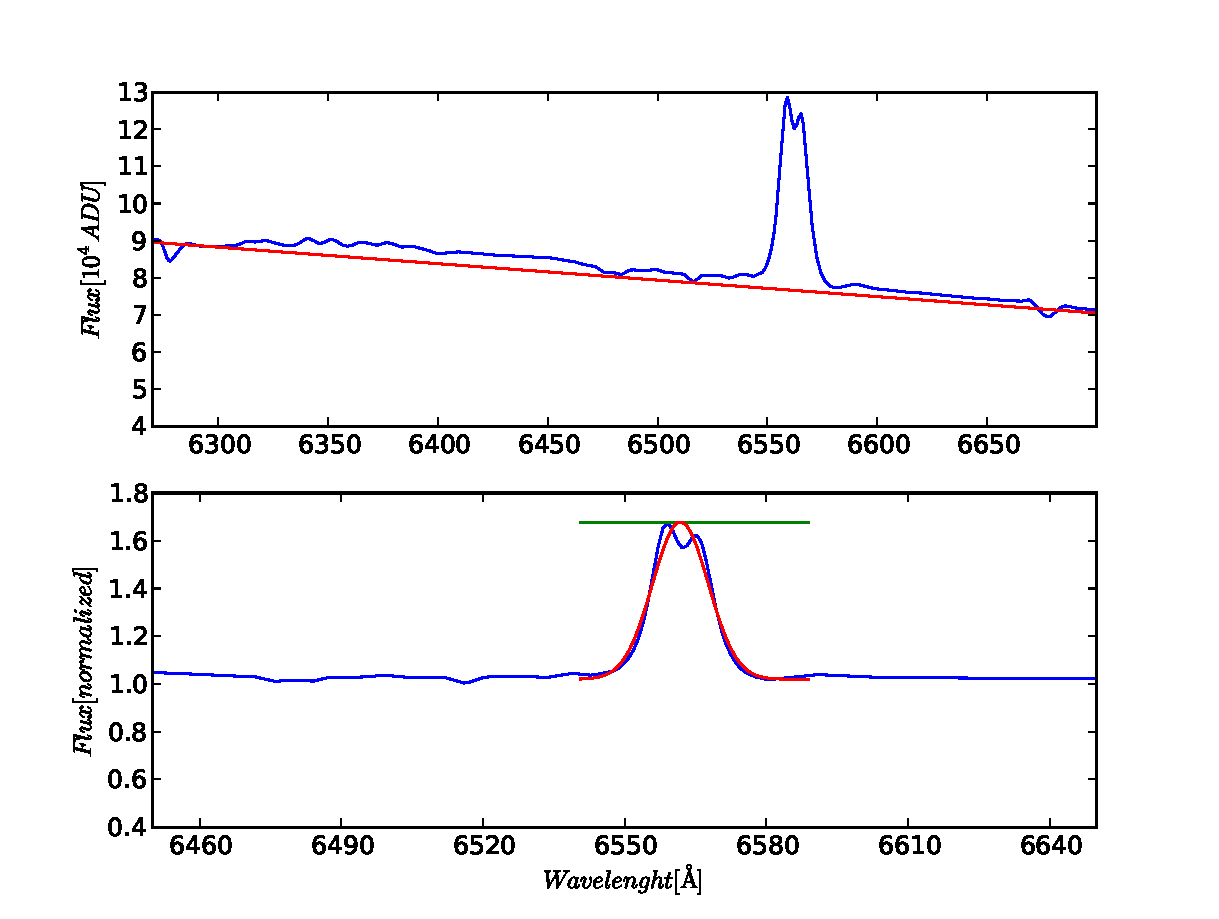
\includegraphics[scale =.8]{figSpecCharCyg60}
        \else
        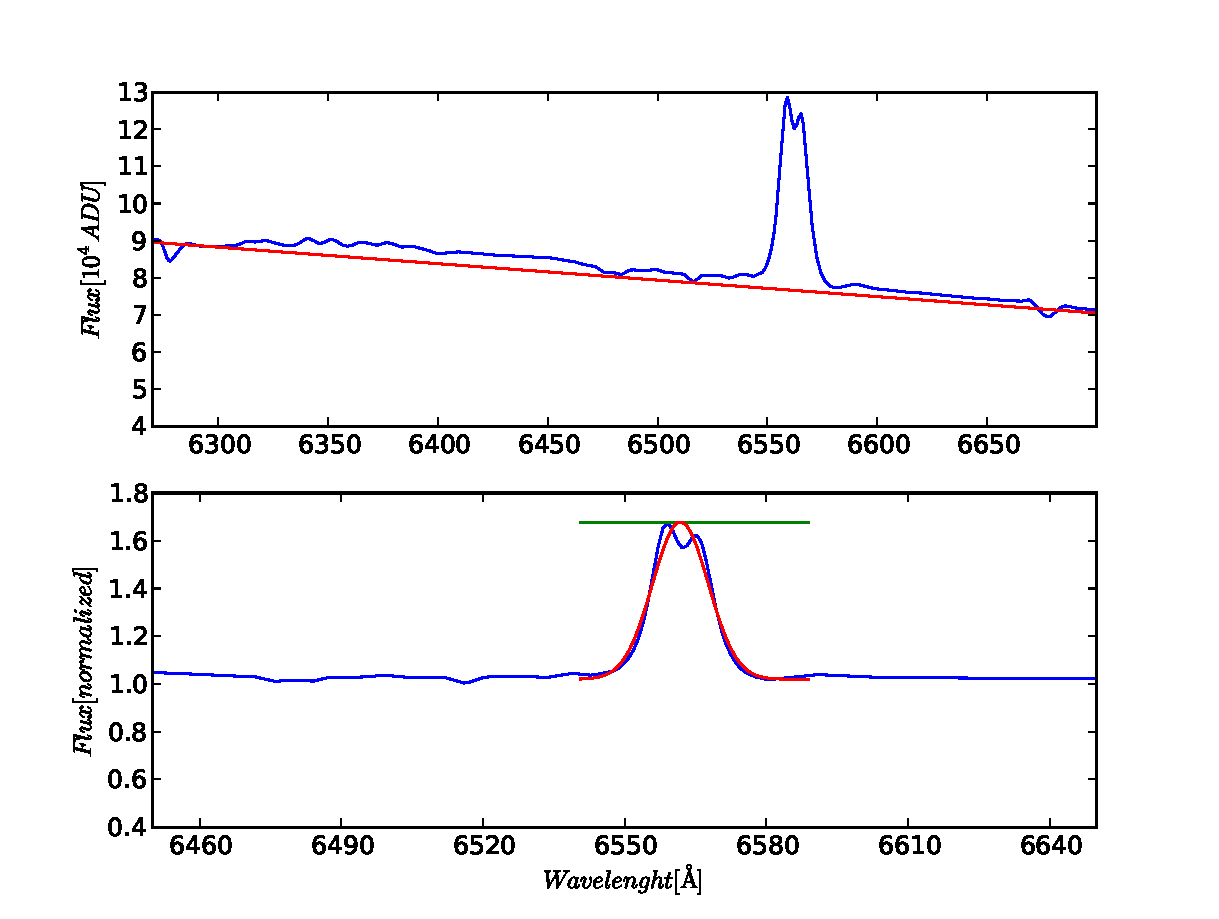
\includegraphics[bb = 92 86 545 742, height=6in]{figSpecCharCyg60}
        \fi
        \caption{Normalized spectrum of Be star 60 Cyg. The top figure
          depicts the continuum fit. The bottom figure shows the
          region (width of the green line) used for extraction. The
          position of the line correspond to the maximum value in the
          region of $50\AA$. The gaussian fit is in red.}
        \label{FigSpecChar}
      \end{center}
    \end{figure}

   \begin{figure}[!htbp]
      \begin{center}
        \leavevmode
        \ifpdf
        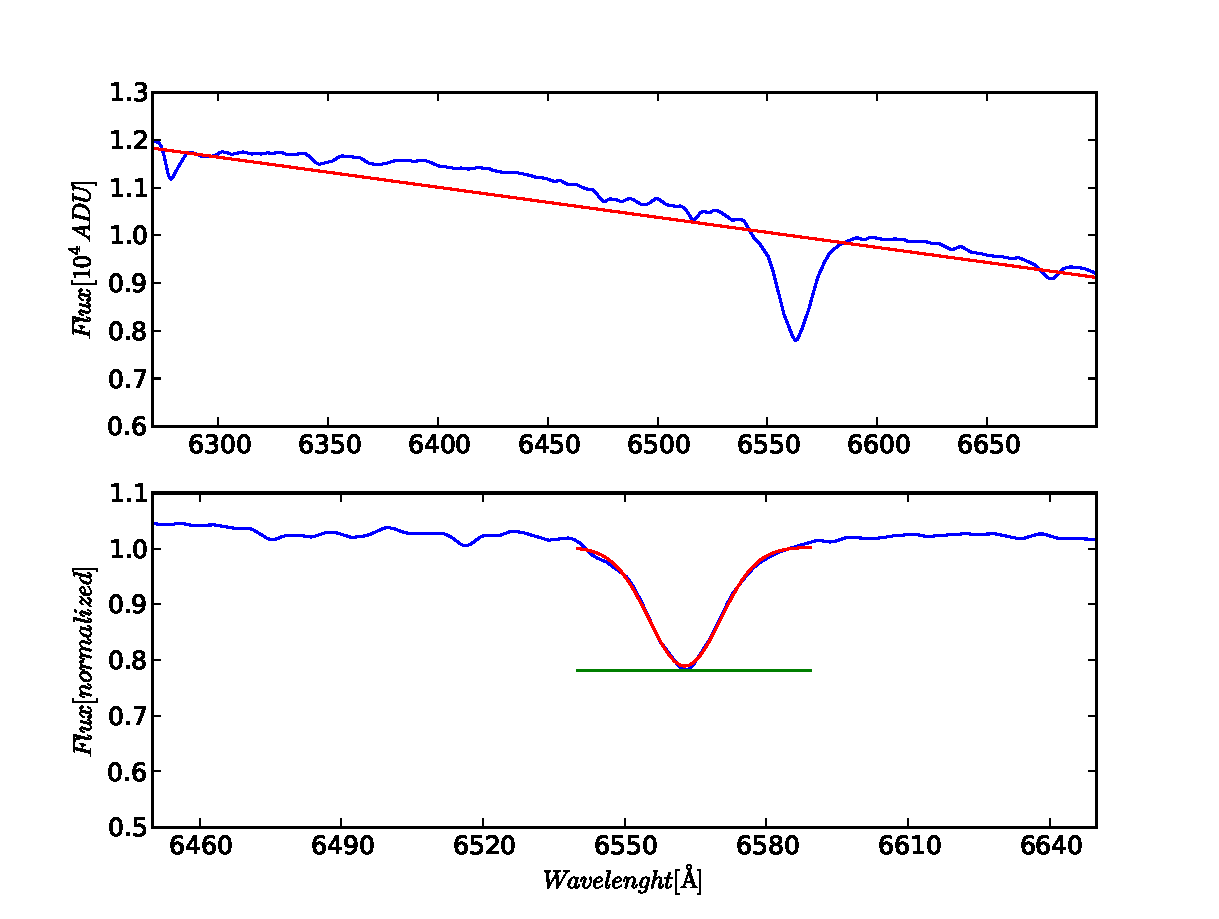
\includegraphics[scale =.8]{figSpecCharhd216057}
        \else
        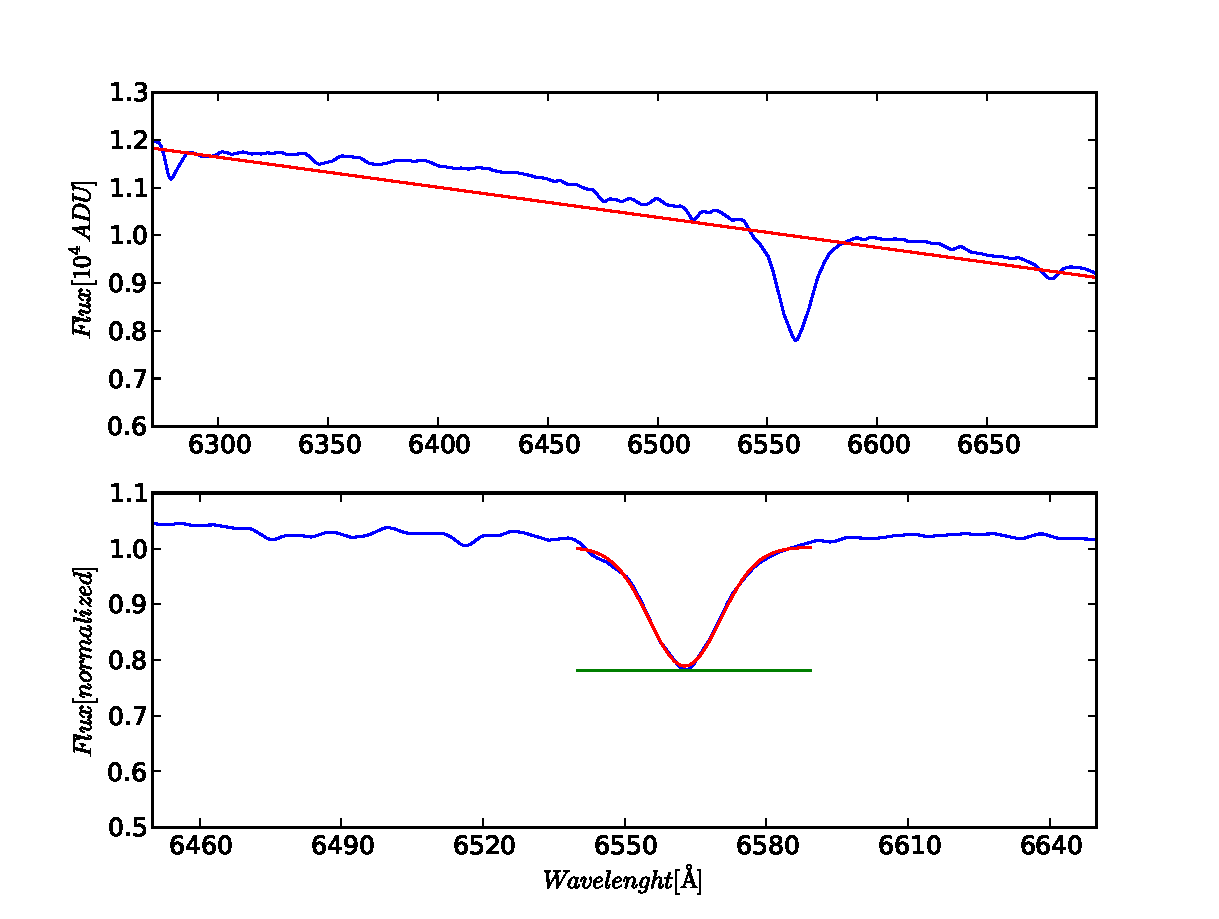
\includegraphics[bb = 92 86 545 742, height=6in]{figSpecCharhd216057}
        \fi
        \caption{Normalized spectrum of Be star HR 8682. The top
          figure depicts the continuum fit. The bottom figure shows
          the region (width of the green line) used for
          extraction. The position of the line correspond to the
          maximum value in the region of $50\AA$. The gaussian fit is
          in red.}
        \label{FigSpecChar}
      \end{center}
    \end{figure}


\clearpage

% The script was written to normalize the spectrum and extract the line
% characteristic value. This program also plots the results of the
% process as it is shown on previous picture. The function used to
% extract the line characteristic value is below.



\subsection{Data Mining}
Classification was performed using weka software with algoritm J48
described in the chapter \ref{chap:dataMining}. Trainning set had 183
and testing set 178314 items. The excerpt from these files follows.

\begin{lstlisting}
@RELATION STAR-B-BE
@ATTRIBUTE name STRING
@ATTRIBUTE alpha NUMERIC
@ATTRIBUTE grp {be,o}
@DATA
10_cas,-0.822196556626,be
11_cyg,1.68689566629,be
\end{lstlisting}

\begin{lstlisting}
@RELATION STAR-B-BE
@ATTRIBUTE name STRING
@ATTRIBUTE alpha NUMERIC
@ATTRIBUTE grp {be,o}
@DATA	 
spSpec-53228-1884-001	-0.584628294569	 ?
spSpec-53228-1884-002	-0.877184482566	 ?
\end{lstlisting}

The attribute \textrm{grp} is known for the trainnig set but uknown
for testing set. The classification process fills this information
based on decision tree created during learning phase. To automte the
process command line verson of weka software was used.

\begin{lstlisting}
  java -classpath weka.jar
  weka.classifiers.meta.FilteredClassifier -F
  weka.filters.unsupervised.attribute.RemoveType -W
  weka.classifiers.trees.J48 -t $1 -T $2 -p 1
\end{lstlisting}


\subsection{Results}

Because only one parameter (H$\alpha$) was used, the decision tree is
very simple. If the value of the parametr is greater than $-0.464633$
the object is considered to be a Be star. If the values in the range
of $-0.676474$ and $-0.464633$ it is considered to be non Be star (no
further restriction was assert on the \textrm{other} group). It imply
that according to classifier the Be star is an object with extreme
values in H$\alpha$ line. This outcome does not oppose our
undestanding of these kind of objects.


\begin{lstlisting}
  J48 pruned tree
------------------
alpha <= -0.464633
|   alpha <= -0.676474: be (45.0/18.0)
|   alpha > -0.676474: o (46.0/5.0)
alpha > -0.464633: be (92.0/16.0)
\end{lstlisting}

\begin{lstlisting}
  === Summary ===
Correctly Classified Instances         142               77.5956 %
Incorrectly Classified Instances        41               22.4044 %
Kappa statistic                          0.5078
Mean absolute error                      0.3215
Root mean squared error                  0.4083
Relative absolute error                 66.4104 %
Root relative squared error             83.0045 %
Total Number of Instances              183     
\end{lstlisting}

\begin{lstlisting}
  === Confusion Matrix ===
 Be     O   <-- classified as
 102    6 |   Be
  35   40 |   Othres
\end{lstlisting}

Confusion Matrix indicates that the classifier is much better in
predicting Be stars (102/6 correct assigments) then in predicting
results in the \textrm{others} group where there are just 40/35 right
assigments.

Spectra of some of the objects classified as Be stars are presented
here. 


   \begin{figure}[!htbp]
      \begin{center}
        \leavevmode
        \ifpdf
        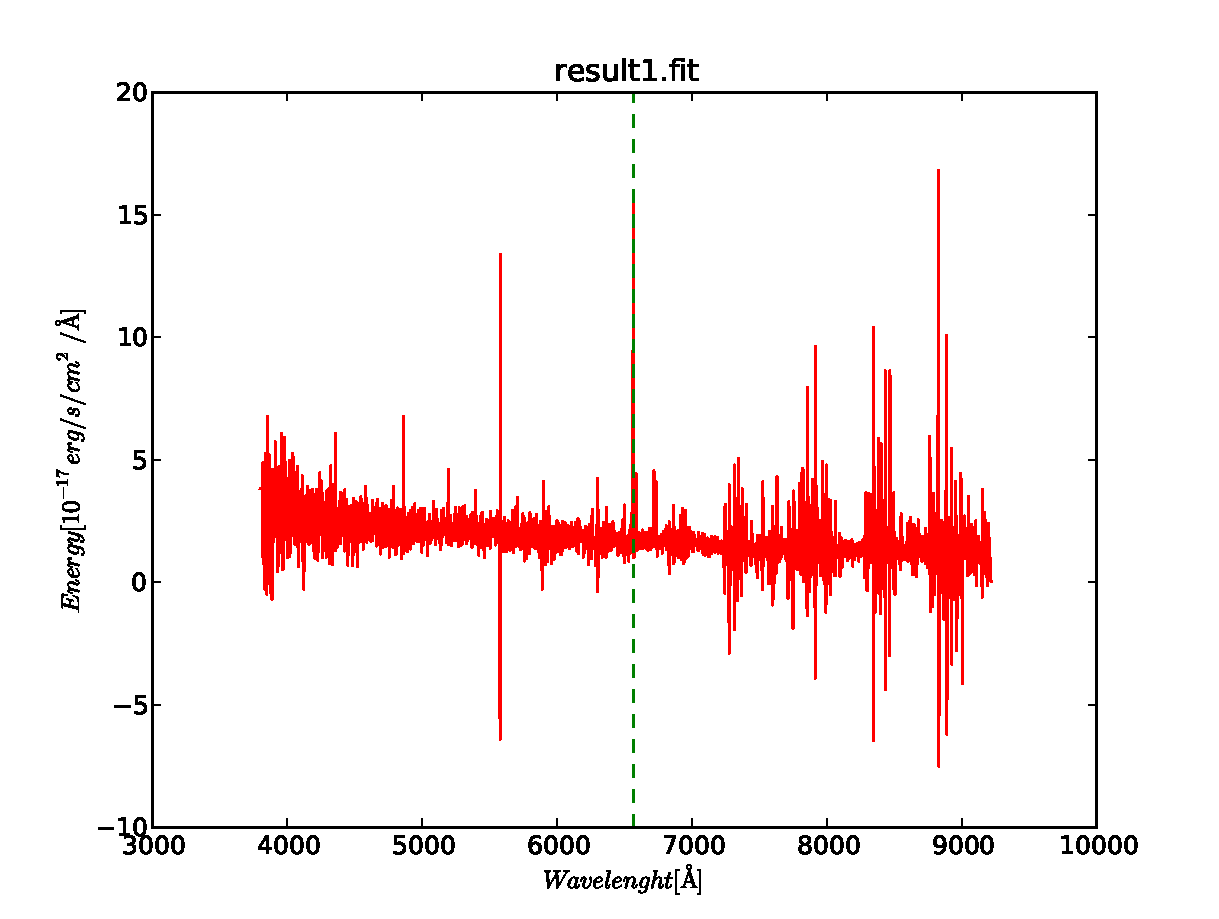
\includegraphics[scale =.8]{result1}
        \else
        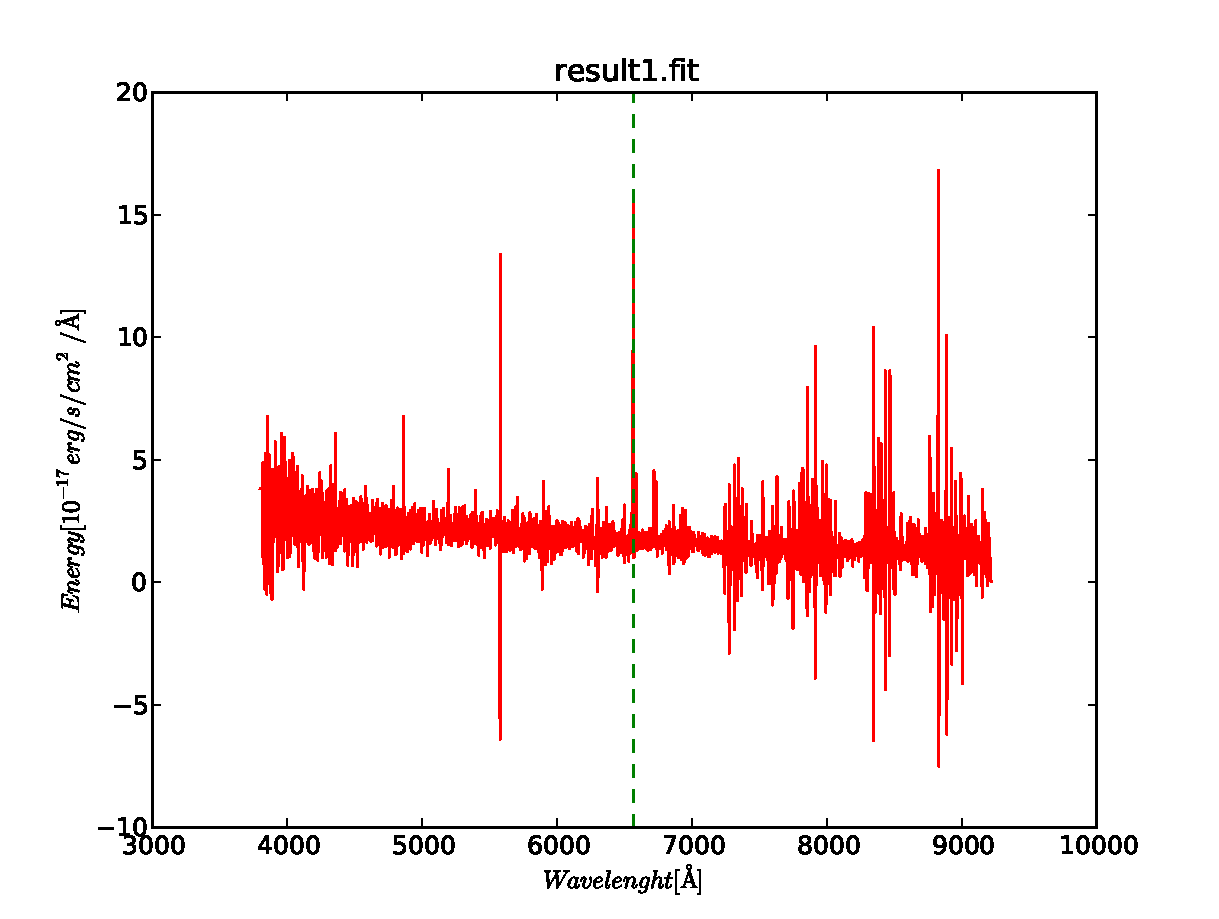
\includegraphics[bb = 92 86 545 742, height=6in]{result1}
        \fi
        \caption{Spectrum of }
        \label{FigResult1}
      \end{center}
    \end{figure}

   \begin{figure}[!htbp]
      \begin{center}
        \leavevmode
        \ifpdf
        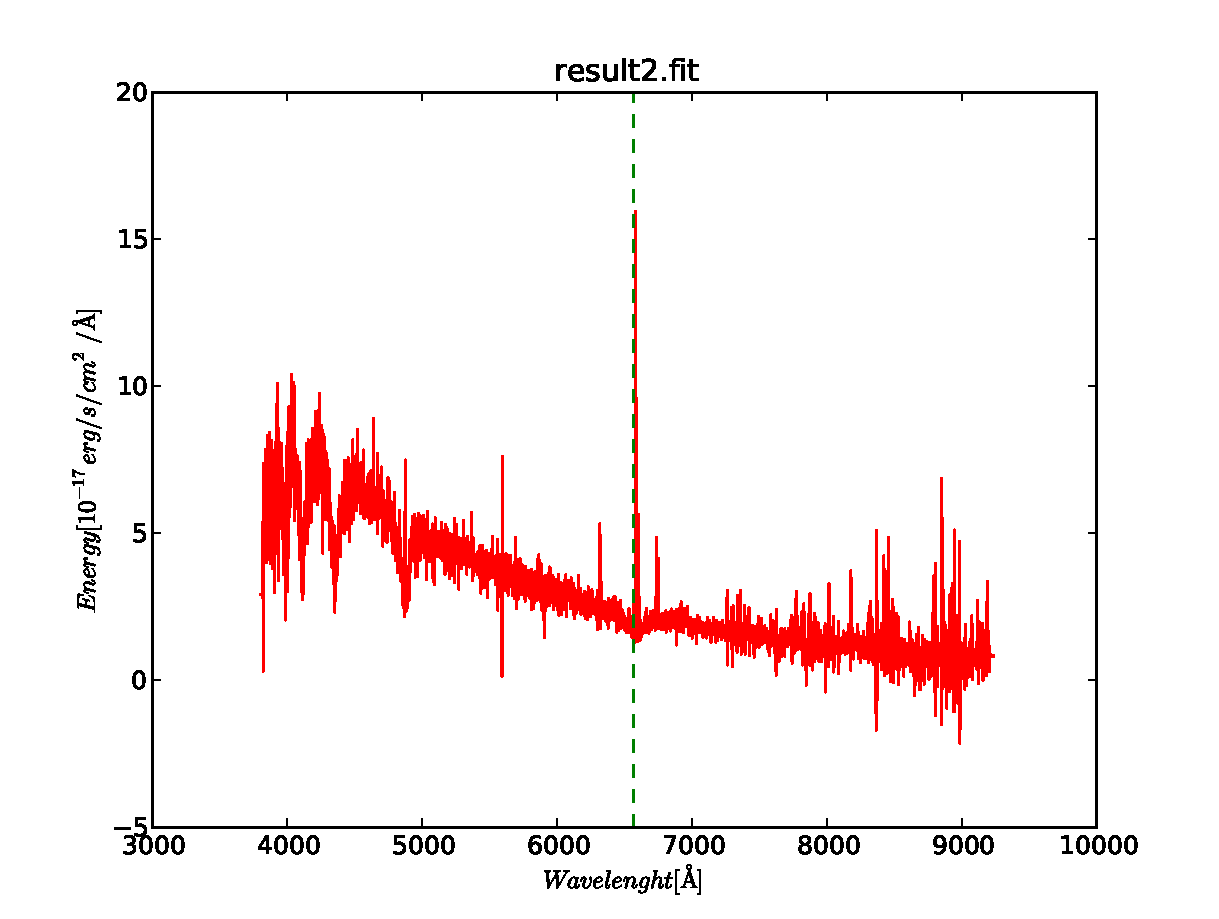
\includegraphics[scale =.8]{result2}
        \else
        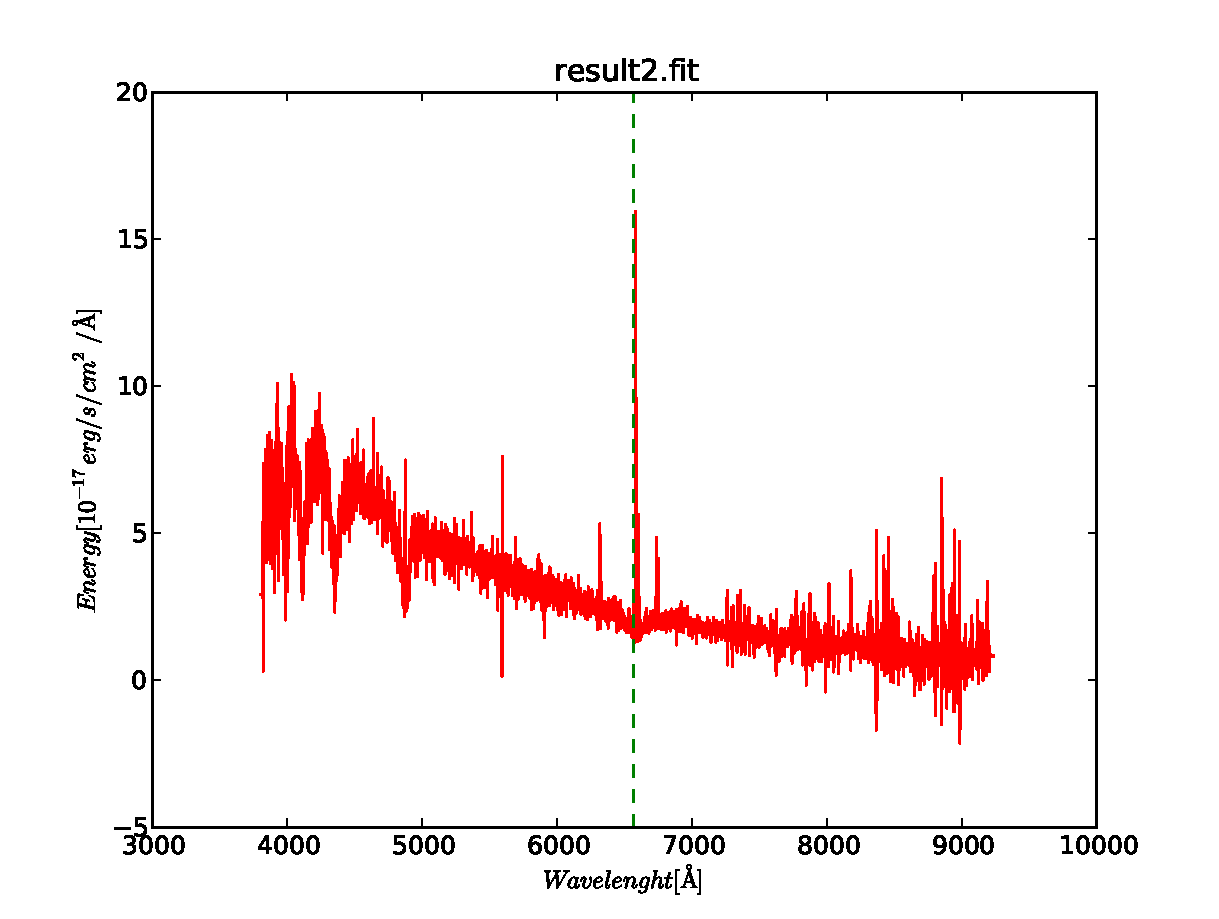
\includegraphics[bb = 92 86 545 742, height=6in]{result2}
        \fi
        \caption{Spectrum of }
        \label{FigResult2}
      \end{center}
    \end{figure}

   \begin{figure}[!htbp]
      \begin{center}
        \leavevmode
        \ifpdf
        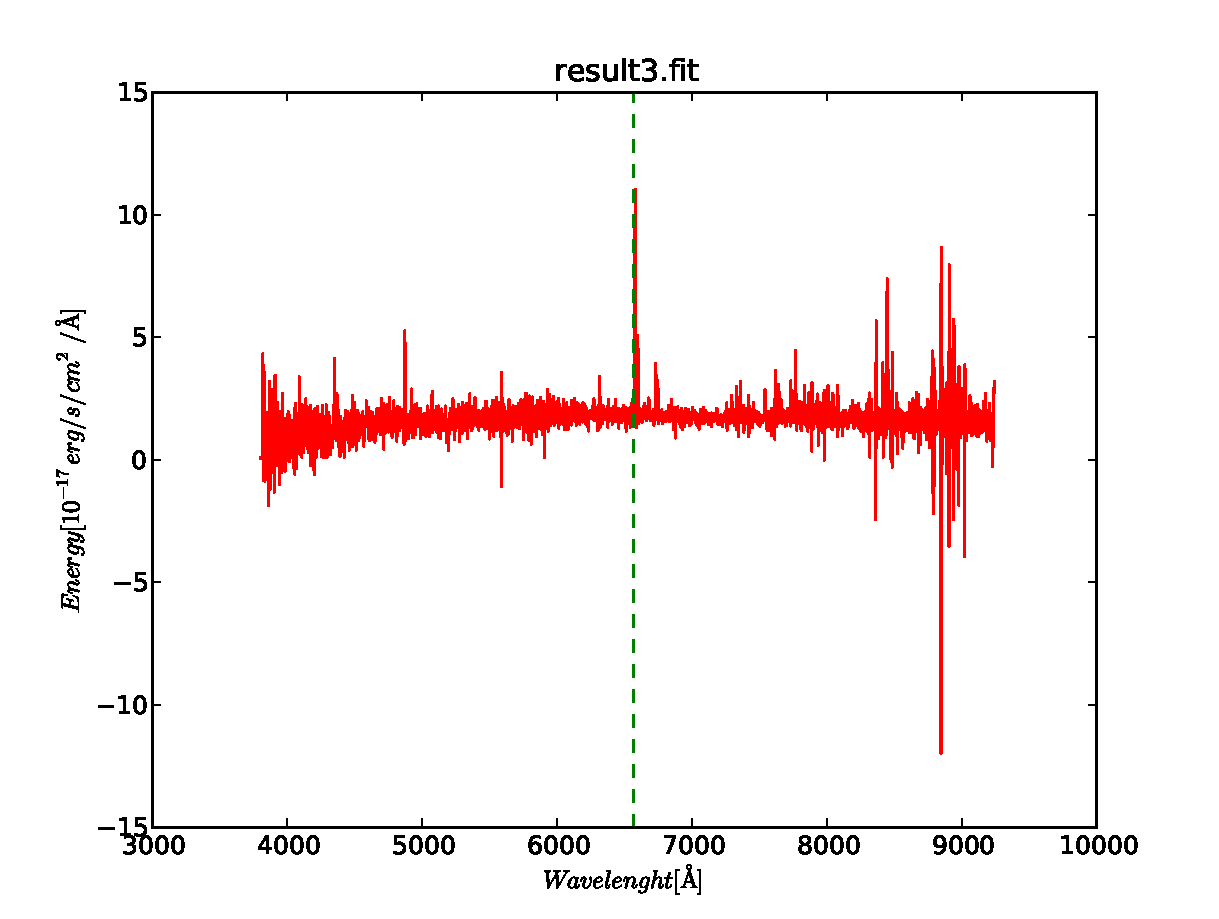
\includegraphics[scale =.8]{result3}
        \else
        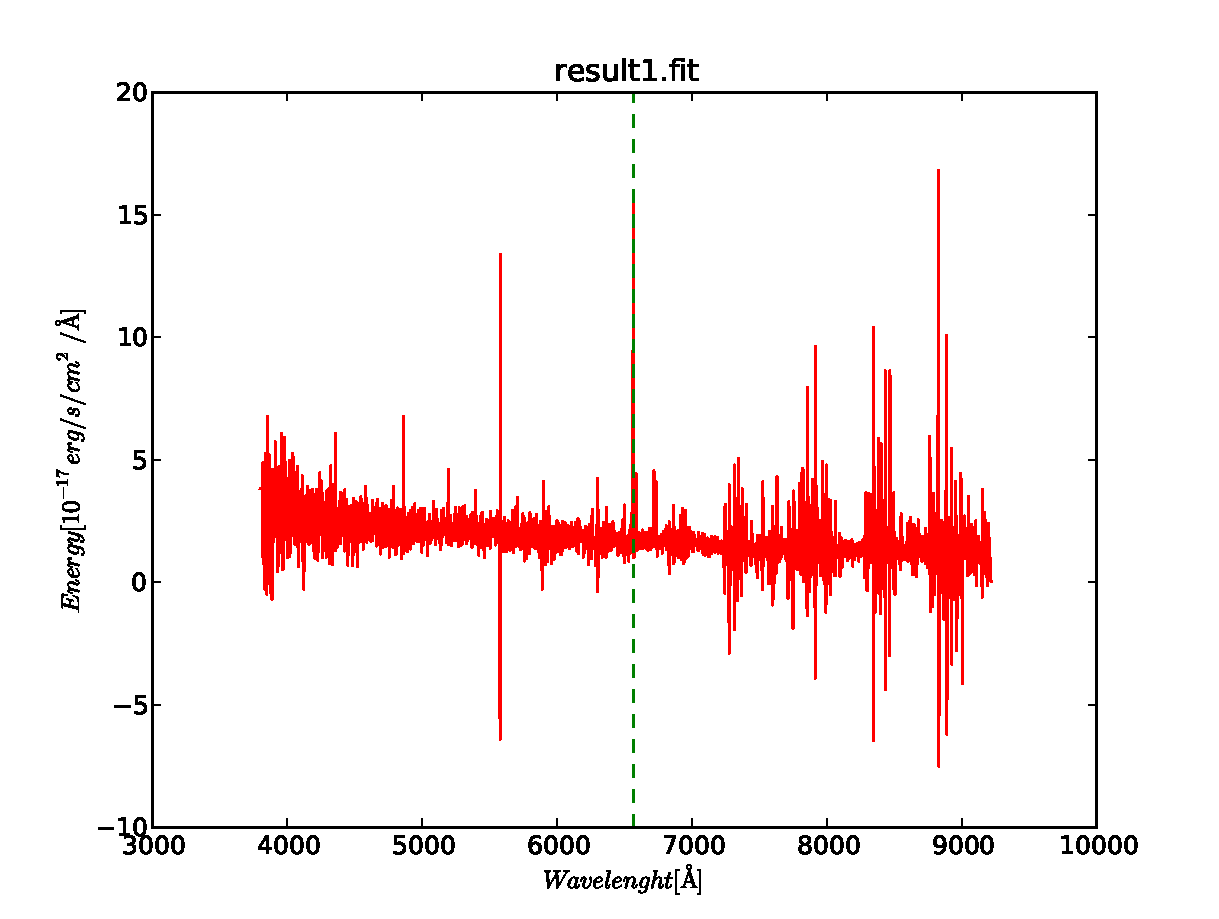
\includegraphics[bb = 92 86 545 742, height=6in]{result1}
        \fi
        \caption{Spectrum of }
        \label{FigResult3}
      \end{center}
    \end{figure}

% Samples of Be Stars           
 
    For comparison there are spectra of know Be stars. It is clear
    that the profile of the H$\alpha$ line is complex and just one
    parameter cannot possibly express it's characteristic. More
    advaced description such as Wavelets coeffiction or theoretical
    models of the line is needed if we want to create realiable
    process for indentifying Be stars.

   \begin{figure}[!htbp]
      \begin{center}
        \leavevmode
        \ifpdf
        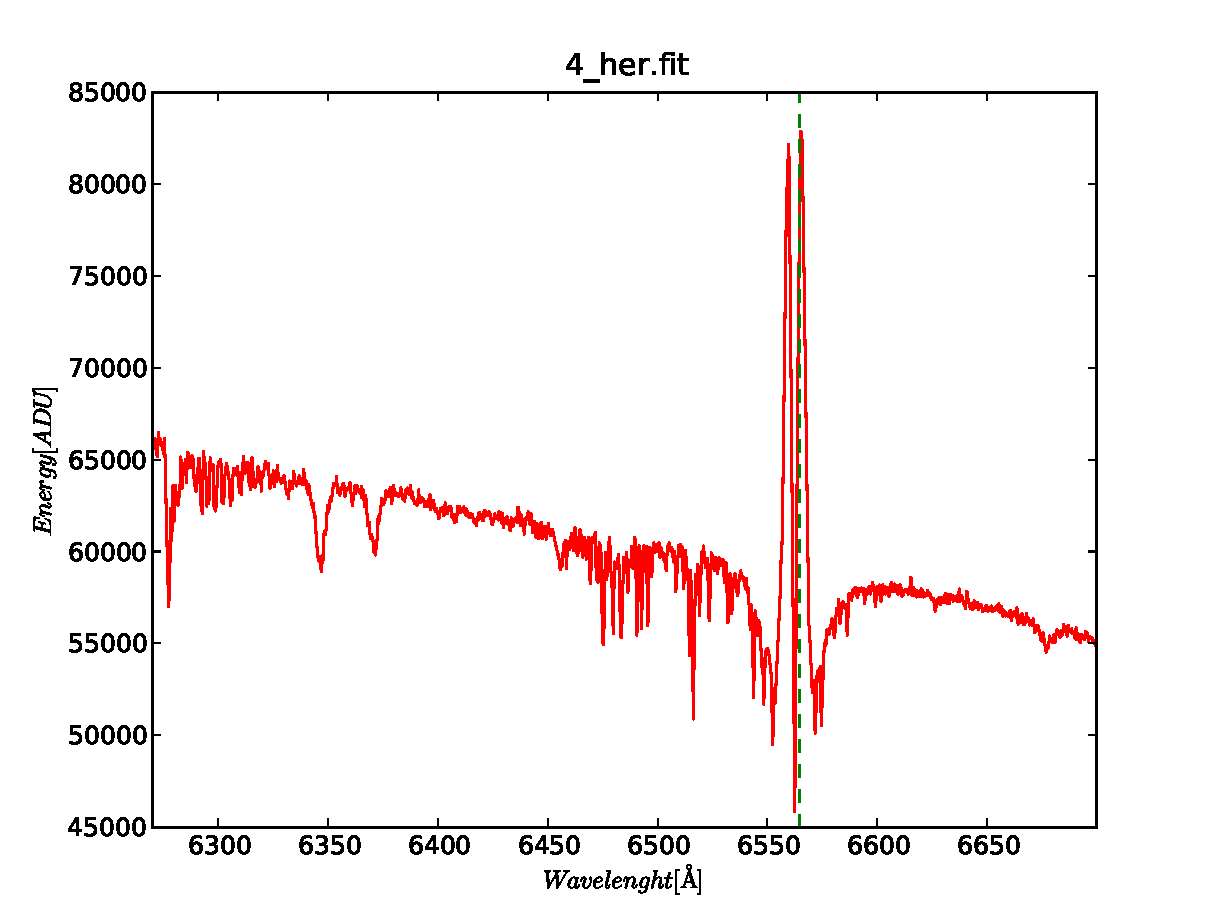
\includegraphics[scale =.8]{be1_4_her}
        \else
        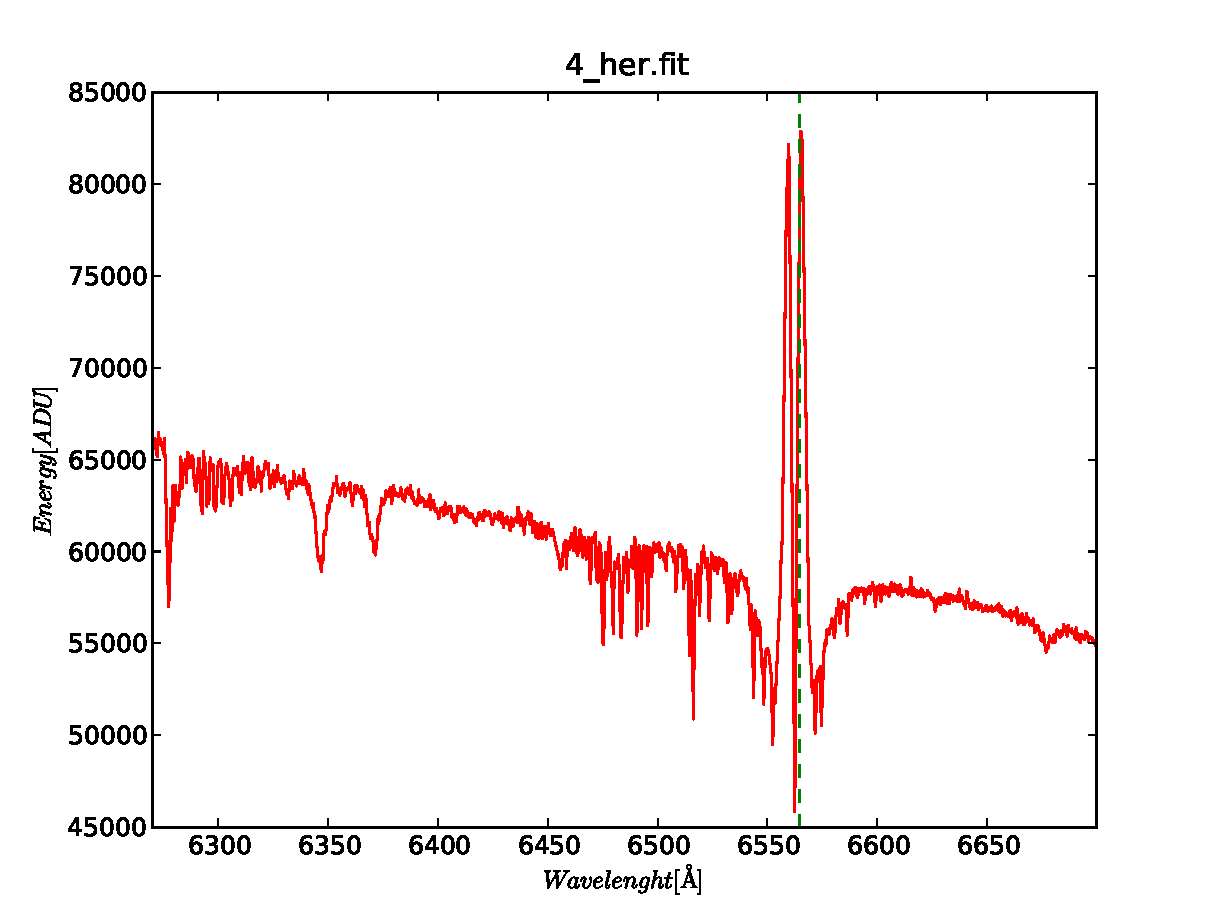
\includegraphics[bb = 92 86 545 742, height=6in]{be1_4_her}
        \fi
        \caption{Spectrum of 4 Her. Be star. Spectral Type B9pe.  }
        \label{FigBe1}
      \end{center}
    \end{figure}

   \begin{figure}[!htbp]
      \begin{center}
        \leavevmode
        \ifpdf
        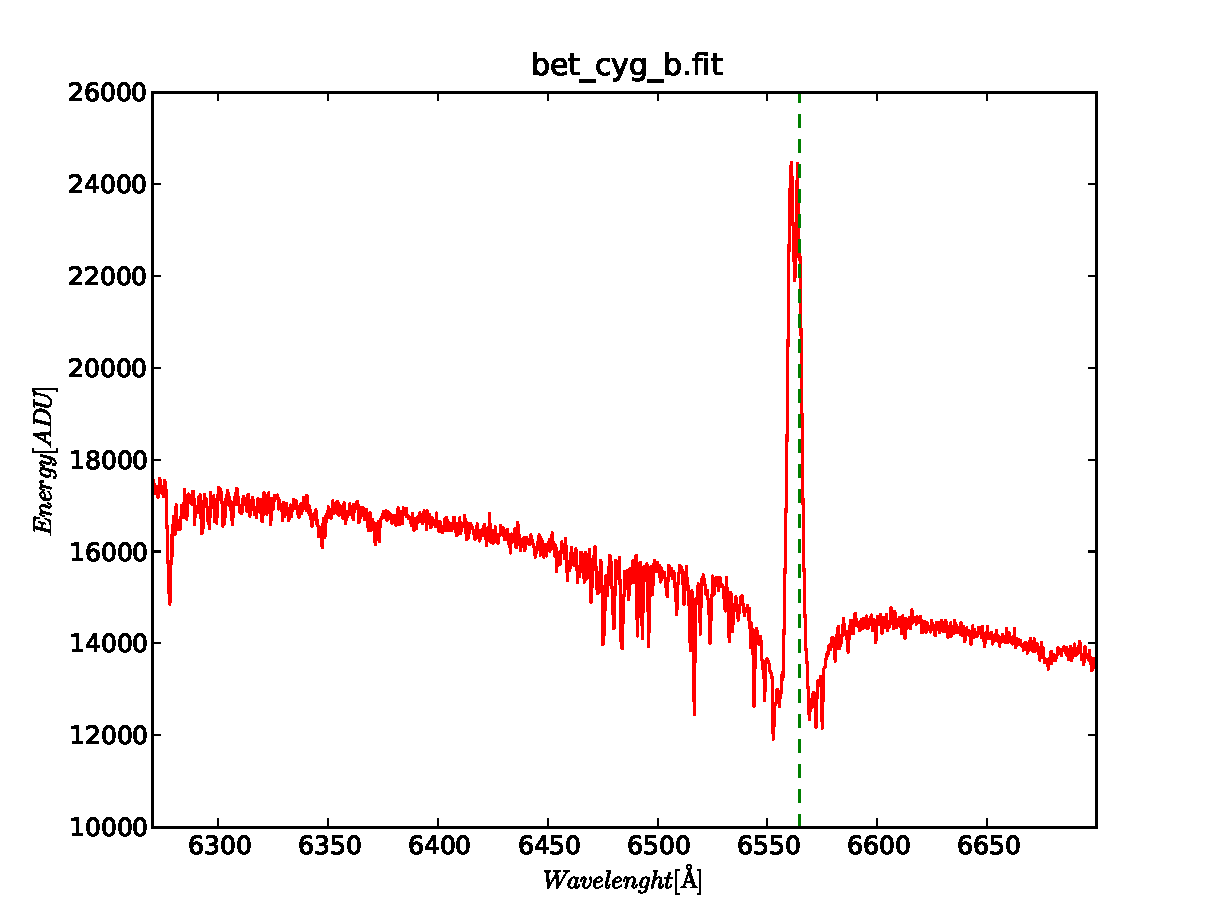
\includegraphics[scale =.8]{be4_bet_cyg_b}
        \else
        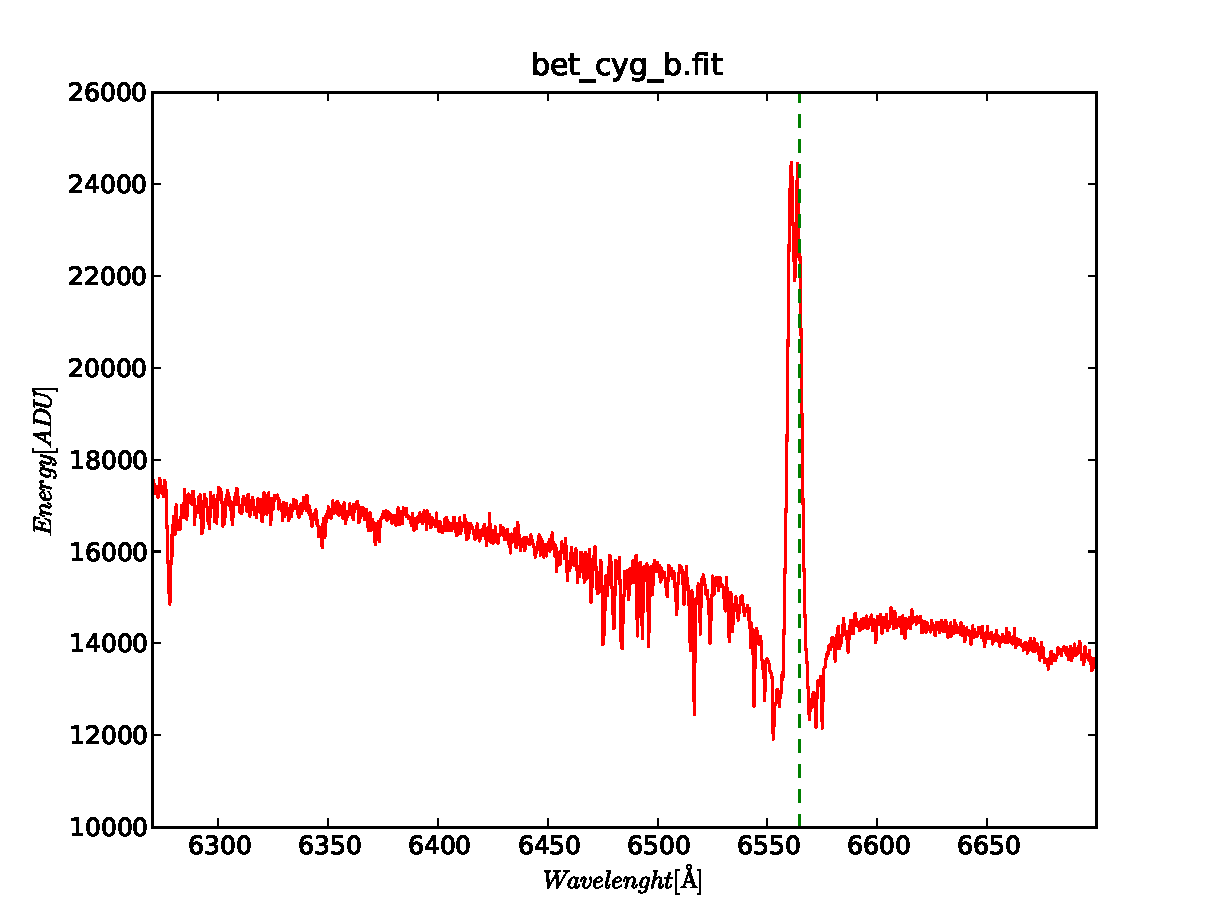
\includegraphics[bb = 92 86 545 742, height=6in]{be4_bet_cyg_b}
        \fi
        \caption{Spectrum of HR 7418 (Albireo B). A fast-rotating Be
          star, with an equatorial rotational velocity of at least 250
          kilometers per second. Its surface temperature has been
          spectroscopically estimated to be about 13.200 K. Spectral
          Type B8Ve. }
        \label{FigBe4}
      \end{center}
    \end{figure}

   \begin{figure}[!htbp]
      \begin{center}
        \leavevmode
        \ifpdf
        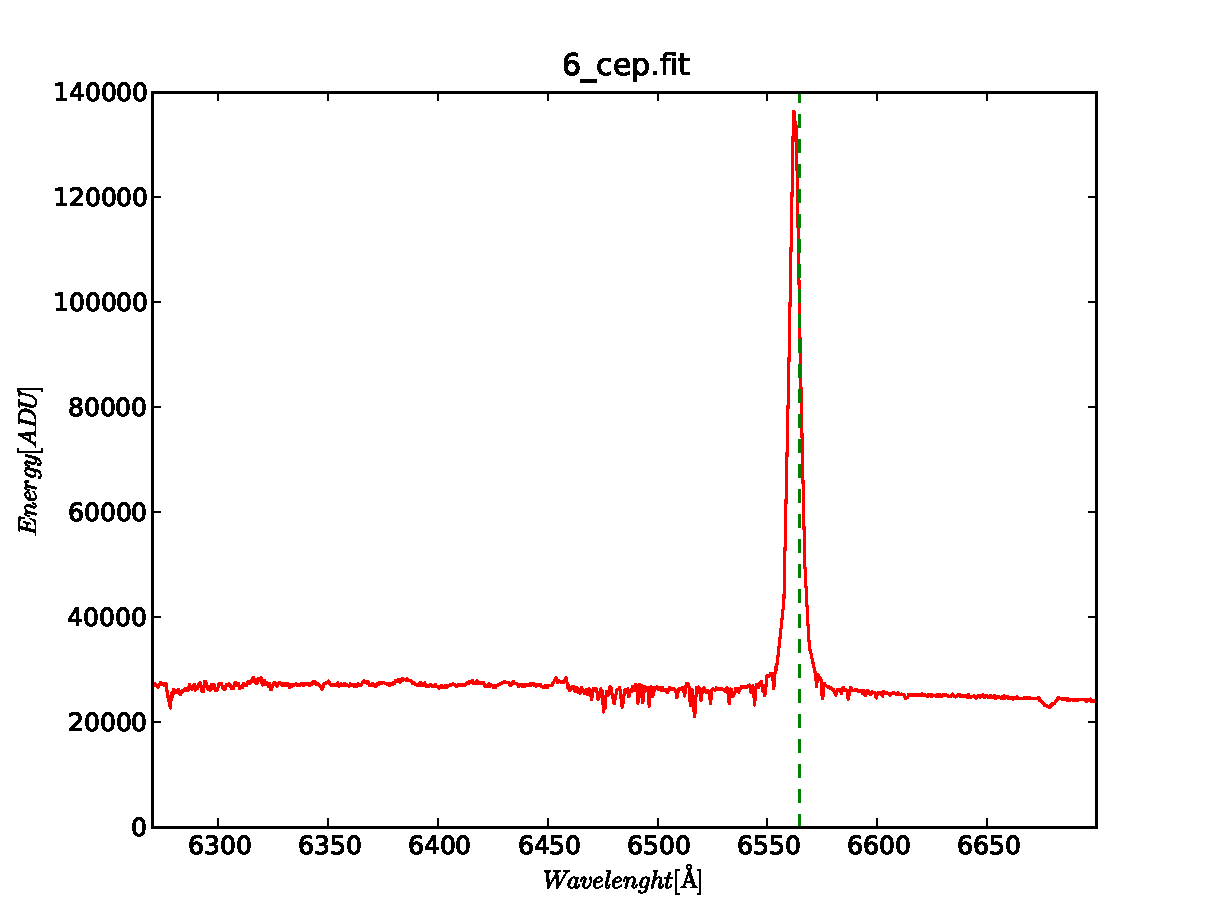
\includegraphics[scale =.8]{be3_6_cep}
        \else
        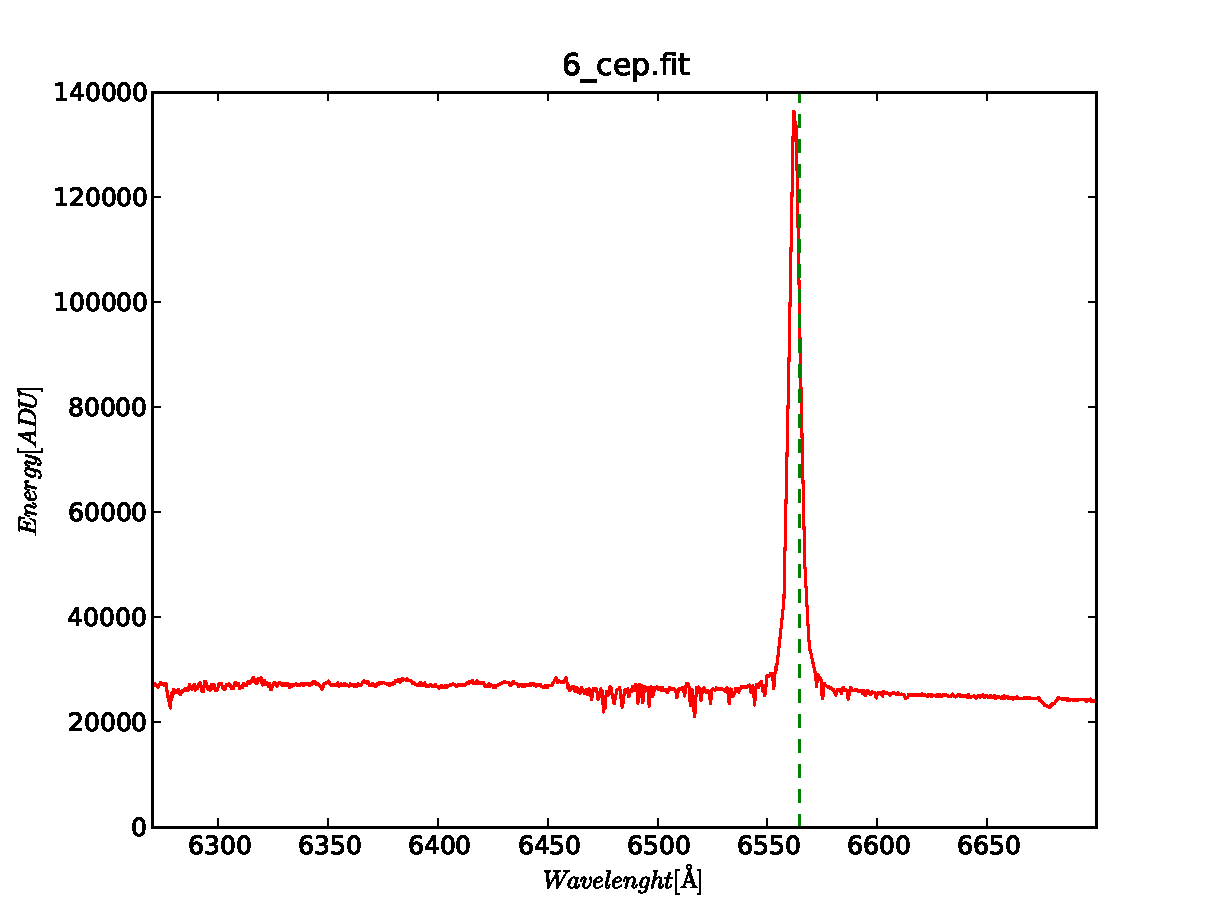
\includegraphics[bb = 92 86 545 742, height=6in]{be3_6_cep}
        \fi
        \caption{Spectrum of 6 Cepheus. Be star. Spectral Type B3IVe.}
        \label{FigBe3}
      \end{center}
    \end{figure}



\clearpage


\subsection{Conclusion}

The harvesting of large-scale of spectral data is challenging but
solvable problem. The technology of Virual Observatory offers solid
background for data discovery and retrieval. The whole process can be
automated using UN*X like approach of small and single purpose scripts
or programs. The last stage of choosing the right characteristics and
Data Mining method is even more complex task requiring deep
understanding of the researched phenomenas and Machine Learnig theory
and technology. The possible solution can be based on cooperation
between experts in scientific and computer science field. Without such
collaboration we are missing lots of opportunities.



% mad2
=== Run information ===

Scheme:       weka.classifiers.trees.J48 -C 0.25 -M 2
Relation:     STAR-BE-O-weka.filters.unsupervised.attribute.Remove-R1
Instances:    173
Attributes:   4
              max
              width
              mad
              grp
Test mode:    10-fold cross-validation

=== Classifier model (full training set) ===

J48 pruned tree
------------------

max <= -0.18843
|   max <= -0.324763: o (46.0/5.0)
|   max > -0.324763
|   |   max <= -0.255475
|   |   |   mad <= 0.004133: o (2.0)
|   |   |   mad > 0.004133: be (13.0/1.0)
|   |   max > -0.255475
|   |   |   mad <= 0.009862: o (10.0)
|   |   |   mad > 0.009862
|   |   |   |   width <= 7.621593: o (3.0/1.0)
|   |   |   |   width > 7.621593: be (2.0)
max > -0.18843
|   mad <= 0.030316
|   |   max <= -0.091726
|   |   |   width <= 5.286489
|   |   |   |   max <= -0.170022: be (2.0)
|   |   |   |   max > -0.170022: o (3.0)
|   |   |   width > 5.286489: be (9.0)
|   |   max > -0.091726: be (76.0)
|   mad > 0.030316
|   |   max <= 6.917615: o (4.0)
|   |   max > 6.917615: be (3.0)

Number of Leaves  : 	12

Size of the tree : 	23


Time taken to build model: 0.12 seconds

=== Stratified cross-validation ===
=== Summary ===

Correctly Classified Instances         145               83.815  %
Incorrectly Classified Instances        28               16.185  %
Kappa statistic                          0.6529
Mean absolute error                      0.1849
Root mean squared error                  0.3652
Relative absolute error                 39.8819 %
Root relative squared error             75.8919 %
Total Number of Instances              173     

=== Detailed Accuracy By Class ===

               TP Rate   FP Rate   Precision   Recall  F-Measure   ROC Area  Class
                 0.864     0.206      0.88      0.864     0.872      0.882    be
                 0.794     0.136      0.769     0.794     0.781      0.882    o
Weighted Avg.    0.838     0.181      0.839     0.838     0.839      0.882

=== Confusion Matrix ===

  a  b   <-- classified as
 95 15 |  a = be
 13 50 |  b = o
